\documentclass[tikz,border=6pt]{standalone}
\usepackage{pgfplots}
\usepackage{amsmath}
\usepackage{amssymb}
\usetikzlibrary{arrows.meta,positioning,calc,patterns}
\usepgfplotslibrary{groupplots}
\pgfplotsset{compat=1.18}

\begin{document}
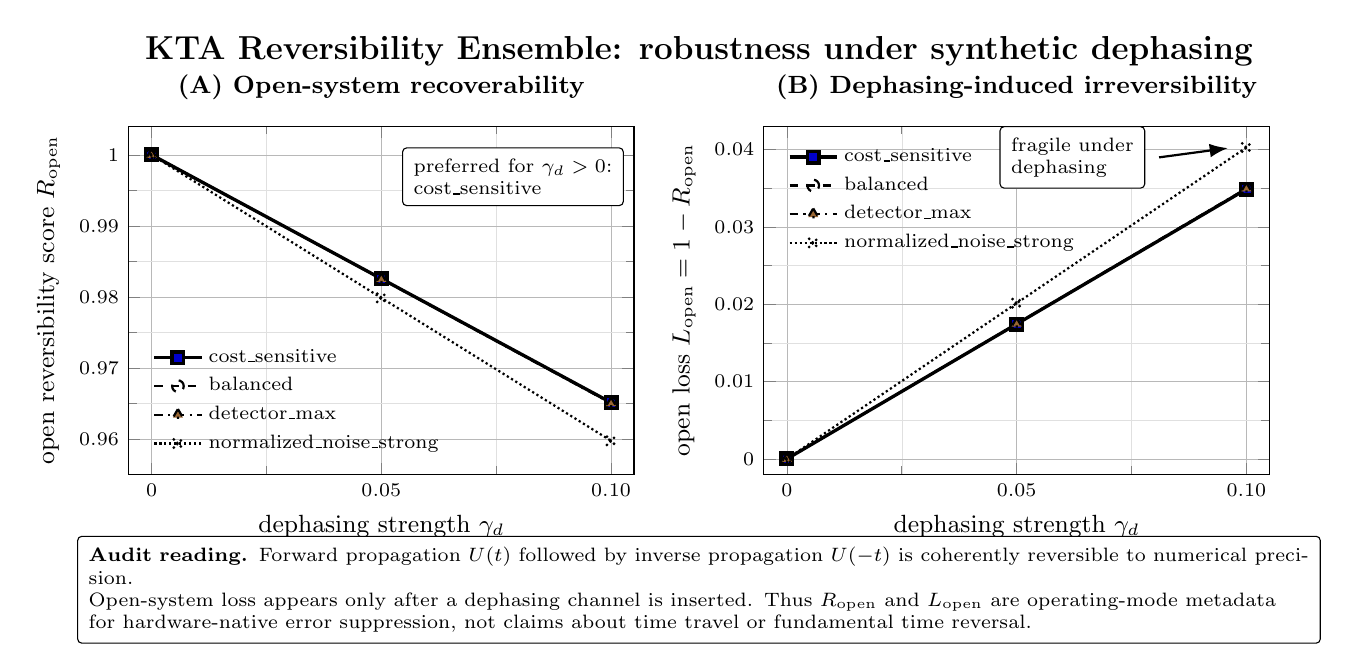
\begin{tikzpicture}[
  note/.style={draw, rounded corners=1.5pt, align=left, font=\scriptsize, fill=white, inner sep=4pt},
  >=Latex
]

\begin{groupplot}[
  group style={group size=2 by 1, horizontal sep=1.65cm},
  width=8.0cm,
  height=6.0cm,
  xmin=-0.005, xmax=0.105,
  xtick={0,0.05,0.10},
  xticklabels={$0$,$0.05$,$0.10$},
  xlabel={dephasing strength $\gamma_d$},
  grid=both,
  minor tick num=1,
  major grid style={line width=.25pt, draw=black!28},
  minor grid style={line width=.15pt, draw=black!12},
  tick label style={font=\scriptsize},
  label style={font=\small},
  title style={font=\small\bfseries, align=center},
  legend style={font=\scriptsize, draw=none, fill=none, cells={anchor=west}}
]

% --- Panel A: Reversibility score ---
\nextgroupplot[
  title={(A) Open-system recoverability},
  ylabel={open reversibility score $R_{\mathrm{open}}$},
  ymin=0.955, ymax=1.004,
  ytick={0.96,0.97,0.98,0.99,1.00},
  legend pos=south west
]

\addplot+[black, very thick, mark=square*, mark size=2.1pt]
coordinates {(0,1.0) (0.05,0.9825568366) (0.10,0.9651136731)};
\addlegendentry{cost\_sensitive}

\addplot+[black, thick, dashed, mark=o, mark size=2.1pt]
coordinates {(0,1.0) (0.05,0.9825316755) (0.10,0.9650633511)};
\addlegendentry{balanced}

\addplot+[black, thick, dash dot, mark=triangle*, mark size=2.1pt]
coordinates {(0,1.0) (0.05,0.9825100916) (0.10,0.9650201831)};
\addlegendentry{detector\_max}

\addplot+[black, thick, densely dotted, mark=x, mark size=2.5pt]
coordinates {(0,1.0) (0.05,0.9798611513) (0.10,0.9597223027)};
\addlegendentry{normalized\_noise\_strong}


\node[note, anchor=north east] at (rel axis cs:0.98,0.94) {preferred for $\gamma_d>0$:\\cost\_sensitive};

% --- Panel B: Open loss ---
\nextgroupplot[
  title={(B) Dephasing-induced irreversibility},
  ylabel={open loss $L_{\mathrm{open}}=1-R_{\mathrm{open}}$},
  ymin=-0.002, ymax=0.043,
  scaled y ticks=false,
  ytick={0,0.01,0.02,0.03,0.04},
  yticklabels={$0$,$0.01$,$0.02$,$0.03$,$0.04$},
  legend pos=north west
]

\addplot+[black, very thick, mark=square*, mark size=2.1pt]
coordinates {(0,0.0000000000000002620) (0.05,0.0174431634) (0.10,0.0348863269)};
\addlegendentry{cost\_sensitive}

\addplot+[black, thick, dashed, mark=o, mark size=2.1pt]
coordinates {(0,0.0000000000000002265) (0.05,0.0174683245) (0.10,0.0349366489)};
\addlegendentry{balanced}

\addplot+[black, thick, dash dot, mark=triangle*, mark size=2.1pt]
coordinates {(0,0.0000000000000002887) (0.05,0.0174899084) (0.10,0.0349798169)};
\addlegendentry{detector\_max}

\addplot+[black, thick, densely dotted, mark=x, mark size=2.5pt]
coordinates {(0,0.0000000000000002087) (0.05,0.0201388487) (0.10,0.0402776973)};
\addlegendentry{normalized\_noise\_strong}

\draw[->, thick] (axis cs:0.081,0.039) -- (axis cs:0.096,0.0402);
\node[note, anchor=east] at (axis cs:0.078,0.039) {fragile under\\dephasing};

\end{groupplot}

% Overall title
\node[font=\large\bfseries, align=center] at ($(group c1r1.north east)!0.5!(group c2r1.north west)+(0,0.95)$)
{KTA Reversibility Ensemble: robustness under synthetic dephasing};

% Bottom method note
\node[note, anchor=north, text width=15.5cm] at ($(group c1r1.south east)!0.5!(group c2r1.south west)+(0,-0.78)$) {
\textbf{Audit reading.} Forward propagation $U(t)$ followed by inverse propagation $U(-t)$ is coherently reversible to numerical precision.\\
Open-system loss appears only after a dephasing channel is inserted. Thus $R_{\mathrm{open}}$ and $L_{\mathrm{open}}$ are operating-mode metadata for hardware-native error suppression, not claims about time travel or fundamental time reversal.
};

\end{tikzpicture}
\end{document}
